\documentclass[a4paper,USenglish]{lites}
  %for A4 paper format use option "a4paper"
  %for british hyphenation rules use option "UKenglish", for american hyphenation rules use option "USenglish"
 % for section-numbered lemmas etc., use "numberwithinsect"
 
\usepackage{microtype}%if unwanted, comment out or use option "draft"
\usepackage{textcomp}

% Citation style
\usepackage[sort&compress,numbers]{natbib}	


\usepackage{xspace}

%\graphicspath{{./graphics/}}%helpful if your graphic files are in another directory

\bibliographystyle{plain}% the recommended bibstyle
%\bibliographystyle{abbrv}% the recommended bibstyle

%\usepackage{graphicx}
\usepackage[super]{nth}





\newcommand{\ceiling}[1]{\left\lceil{#1}\right\rceil}
\newcommand{\floor}[1]{\left\lfloor{#1}\right\rfloor}
\newcommand{\setof}[1]{\left\{{#1}\right\}}
\newcommand{\set}[2]{\{{#1}\mid{#2}\}}

\newcommand{\jj}[1]{\textcolor{blue}{jj: #1 : endjj}}

%%%%%%%%%%%%%%%
 \def\myendproof{{\ \vbox{\hrule\hbox{%
   \vrule height1.3ex\hskip0.8ex\vrule}\hrule }}\par}
 \renewenvironment{proof}{\noindent{\bf Proof. }}{\myendproof}  
  
  

\papertrue 
\title{A Note on the Period Enforcer Algorithm  for Self-Suspending Tasks}

\author[1]{Jian-Jia Chen}
\author[2]{Bj\"orn B.\ Brandenburg}
\affil[1]{TU Dortmund University, Germany\\
  \texttt{jian-jia.chen@cs.uni-dortmund.de}}
\affil[2]{Max Planck Institute for Software Systems (MPI-SWS)\\
  \texttt{bbb@mpi-sws.org}}
\authorrunning{Chen and Brandenburg} %mandatory. First: Use abbreviated first/middle names. Second (only in severe cases): Use first author plus 'et. al.'

\Copyright{Chen and Brandenburg}%mandatory. LIPIcs license is "CC-BY";  http://creativecommons.org/licenses/by/3.0/

%\subjclass{MANDATORY:  Please refer to \url{www.acm.org/about/class/2012}}% mandatory: Please choose 2012 ACM classifications from http://www.acm.org/about/class/2012 . E.g., cite as "Integrated circuits". 
%\keywords{MANDATORY: Please provide 1--5 keywords as a comma-separated list}% mandatory: Please provide 1-5 keywords
%%%%%%%%%%%%%%%%%%%%%%%%%%%%%%%%%%%%%%%%%%%%%%%%%%%%%%%%%

%EditorialOffice macros (do not touch as author)%%%%%%%%%%%%%%%%%%%%%%%%%%%%%%%%%%%
\Volume{XXX}
\Issue{YYY}
\DateSubmission{Date of submission}
\DateAcceptance{Date of acceptance}
\DatePublished{Date of publishing}
\SectionAreaEditor{LITES section area editor}
\DOI{10.4230/LITES.xxx.yyy.p}
%%%%%%%%%%%%%%%%%%%%%%%%%%%%%%%%%%%%%%%%%%%%%%%%%%%%%%%%%


\begin{document}

\maketitle
\begin{abstract}
The \emph{period enforcer} algorithm for self-suspending real-time tasks is a technique for suppressing the ``back-to-back'' scheduling penalty associated with deferred execution. Originally proposed in 1991, the algorithm has attracted renewed interest in recent years. This note revisits the algorithm in the light of recent developments in the analysis of self-suspending tasks, carefully re-examines and explains its underlying assumptions and limitations, and points out three observations that have not been made in the literature to date: \textbf{(i)}~period enforcement is not strictly superior as it can cause deadline misses in self-suspending task sets that are schedulable without enforcement; \textbf{(ii)}~with current techniques, schedulability analysis of the period enforcer algorithm requires a proper transformation, that is subject to exponential time complexity, of the task set to satisfy the assumptions; and \textbf{(iii)} the period enforcer algorithm is incompatible with all existing analyses of suspension-based locking protocols, and can in fact cause ever-increasing suspension times until a deadline is missed.
\end{abstract}

\section{Introduction} 
This report revists the \emph{period enforcer} algorithm proposed by Rajkumar \cite{Raj:suspension1991} to handle self-suspending real-time tasks. The report briefly reviews the period enforcer algorithm, explains its underlying assumptions and limitations, and discusses how it may be analyzed to correctly determine the schedulability of self-suspending sporadic real-time tasks subject to period enforcement. 

The main contributions of this report are two observations that have not been previously reported in the real-time literature:

\begin{enumerate}
	\item period enforcement can render self-suspending tasks sets unschedulable that are schedulable otherwise (i.e., period enforcement can induce deadline misses); and
	\item with current techniques, schedulability analysis of the period enforcer algorithm requires a task set transformation that is subject to exponential time complexity.
\end{enumerate}

\subsection{Preliminaries}

To date, the real-time literature on self-suspending tasks has focused on two task models: the \emph{dynamic} and the \emph{segmented} (or \emph{multi-segment}) self-suspension model. 
The dynamic self-suspension sporadic task model characterizes each
task $\tau_i$ as a $4$-tuple $(C_i,S_i,T_i,D_i)$: 
$C_i$ denotes the upper bound on the total execution time of any job of $\tau_i$,
$S_i$ denotes the upper bound on the total self-suspension time of any job of $\tau_i$,
$T_i$ denotes the minimum inter-arrival time (or period) of $\tau_i$, and $D_i$ is the relative deadline. The dynamic self-suspension model does not impose a bound on the maximum number of self-suspensions, nor does it make any assumptions as to where during a job's execution self-suspensions occur.

In contrast, the segmented sporadic task model extends the above $4$-tuple by characterizing each self-suspending task as a (fixed) finite linear sequence of computation and suspension intervals. These intervals are represented as a tuple
$(C_{i}^1,S_{i}^1,C_{i}^2,S_{i}^2,...,S_{i}^{m_i-1},C_{i}^{m_i})$, which is composed of $m_i$ computation segments separated by $m_i-1$ suspension intervals. For the simplicity of presentation, we assume that a task $\tau_i$ always starts with a computation segment. The arguments can be easily extended to handle tasks that start with self-suspensions.

The advantage of the dynamic model is that it is more flexible since it does not impose any assumptions on control flow. The advantage of the segmented model is that is allows for more accurate analysis. The period enforcer algorithm and its analysis fundamentally applies (only) to the segmented model.

The central notation in Rajkumar's analysis~\cite{Raj:suspension1991} is a \emph{deferrable task}, which matches our notion of multi-segment tasks.  Specifically, Rajkumar states that:
\begin{quote}
With deferred execution, a task $\tau_i$ can execute its $C_i$ units of execution in discrete amounts $C_i^1, C_i^2$, $\ldots$ with suspension in between $C_i^j$ and $C_i^{j+1}$. \cite[Section 3]{Raj:suspension1991}\footnote{The notation has been altered here for the sake of consistency.} 
\end{quote}
%
Central to Rajkumar's analysis~\cite{Raj:suspension1991} is a \emph{task set transformation} that splits each deferrable task with multiple segments into a corresponding number of single-segment deferrable tasks.  In the words of Rajkumar~\cite[Section 3]{Raj:suspension1991}:

\begin{quote}
	 Without any loss of generality, we shall assume that a task $\tau_i$ can defer its entire execution time but not parts of it. That is, a task $\tau_i$ executes for $C_i$ units with no suspensions once it begins execution. Any task that does suspend after it executes for a while can be considered to be two or more tasks each with its own worst-case execution time. The only difference is that if a task $\tau_i$ is split into two tasks $\tau_i'$ followed by $\tau_i''$, then $\tau_i''$ has the same deadlines as $\tau_i{{'}}$. 
\end{quote}
%
In other words, the transformation can be understood as splitting each self-suspending task into a matching number of non-self-suspending sporadic tasks subject to \emph{release jitter}, which can be easily analyzed with classic fixed-priority response-time analysis~\cite{ABRTW:93}.

It is well known that uncontrolled deferred execution (i.e, release jitter) can impose a scheduling penalty because of the potential for ``back-to-back'' execution~\cite{ABRTW:93}. That is, if a job of a deferrable task that maximally defers its execution is directly followed by a job that executes immediately without deferring its execution, then lower-priority tasks may suffer increased interference. 

The purpose of the period enforcer algorithm is to reduce such penalties for lower-priority tasks without detrimentally affecting the schedulability of self-suspending, higher-priority tasks. The latter aspect --- no detrimental effects for self-suspending tasks --- is captured concisely by Theorem 5 in the original analysis of the period enforcer algorithm \cite{Raj:suspension1991}.
\begin{quote}
{\bf Theorem 5}: A deferrable task that is schedulable under its worst-case conditions is also schedulable under the period enforcer algorithm.  \cite{Raj:suspension1991}
\end{quote}

\subsection{Questions answered in this report}

Theorem 5 in \cite{Raj:suspension1991} provides a very positive result for the analysis of deferrable task sets subject to period enforcement. That is, if the corresponding transformed task set can be shown to be schedulable under fixed-priority scheduling using \emph{any} applicable analysis, then the period enforcer algorithm also provides a feasible schedule. 

However, note that Theorem 5 in \cite{Raj:suspension1991} applies only to the \emph{transformed} task set: recall that, in the original analysis~\cite{Raj:suspension1991}, deferrable tasks are assumed to defer their entire execution time either completely or not at all (but not parts of it).  Therefore, if we would like to use the period enforcer algorithm to handle segmented self-suspending task sets, we first have to answer the following question: ``\emph{Given a set of sporadic segmented self-suspending tasks, what is the corresponding set of (single-segment) deferrable tasks?}'' That is, how do we convert given self-suspension segments into equivalent bounds on release jitter such that we may apply Theorem 5 to conclude that the system remains schedulable despite period enforcement? Unfortunately, the original proposal \cite{Raj:suspension1991} does not provide an answer to this central question. 


In this report, we make two observations pertinent to this question:
\begin{enumerate}
	\item There exist sporadic segmented self-suspending task sets that are schedulable under fixed-priority scheduling without any enforcement, but the corresponding schedule by using the period enforcer algorithm is not feasible. This shows that Theorem 5 in \cite{Raj:suspension1991} has to be  used with care --- it may be applied only in the context of the transformed single-segment deferrable task set, and not in the context of the original segmented self-suspending task set.

	\item Deriving a single-segment deferrable task set corresponding to a given set of sporadic segmented self-suspending tasks in polynomial time is an open problem. Recent findings by Nelissen et al. \cite{ecrts15nelissen} can be applied, but their method takes exponential time.
\end{enumerate}

\section{Deadline Missses Caused by Period Enforcement}
\label{sec:unschedulable}

In this section, we demonstrate with an example that there exist sets of segmented self-suspending sporadic tasks that both \textbf{(i)} are schedulable \emph{without} period enforcement and \textbf{(ii)} are not schedulable under the period enforcer.

Consider a task system with $2$ tasks. Let $C_1 = 2$ and $T_1=D_1=10$ (without self-suspension). Let $C_{2,1} = 1, S_{2,1} = 6, C_{2,2}=1, T_2=D_2=11$. Suppose that we use the rate-monotonic priority assignment, i.e., $\tau_1$ has higher priority than $\tau_2$. This task system is feasible without any enforcement since at most one computation segment of a job of $\tau_2$ can be affected by $\tau_1$. The worst-case response time of task $\tau_2$ is hence $10$. 

Figure \ref{fig:example} is the resulting schedule by using the period enforcer algorithm. The first job of task $\tau_2$ (that arrives at time $0$) is executed as if there is no period enforcement. The second job (that releases at time $11$) of task $\tau_2$ requires some attention to understand how the period enforcer algorithm works. Note that the first computation segment of task $\tau_2$ does not suffer from any deferrable execution (it is postponed due to higher-priority block). Therefore, it is always placed to the ready queue immediately when it arrives and scheduled as early as possible.

Let's now look at the computation segment $C_2^2$ of the second job of task $\tau_2$. This segment is placed back to the ready queue at time $19$ after its self-suspension. Without period enforcement, this computation segment should be executed from $19$ to $20$. However, the period enforcer algorithm intentionally defers this computation segment to ensure \emph{the periodic demand} of the computation segment $C_2^2$. Therefore, this computation segment is \emph{activated} to the ready queue at time $9+T_2=9+11=20$. This results in a deadline miss.\footnote{By using the notations in \cite{Raj:suspension1991}, we have $ET_{2,1}^2=9, ET_{2,2}^2 = \max\{9+11, 19\}=20$. The superscript $^2$ is for denoting the second computation segment of task $\tau_2$.}

Therefore, the above example shows that there exists (at least) a sporadic segmented self-suspending task system that is schedulable under fixed-priority scheduling without any enforcement, but the corresponding schedule by using the period enforcer algorithm is not feasible. In this example, it is also clear that we can pessimistically convert the two computation segments of task $\tau_2$ into two deferrable tasks $\tau_2^1$ and $\tau_2^2$. The deferrable time of task $\tau_2^1$ is $0$, whereas the deferrable time of task $\tau_2^2$ is at most \emph{$9$}. With the above conversion, we can clearly see that the deferrable task set $\{\tau_1, \tau_2^1, \tau_2^2\}$ is in fact not schedulable by the rate-monotonic priority assignment since we can release a job of $\tau_1$ together with a job of $\tau_2^2$ (after its worst-case deferrable time).

\section{How to Convert to the Corresponding Deferrable Task Set}
\label{sec:convert}

The example in Section \ref{sec:unschedulable} can be easily converted to a corresponding deferrable task set. However, it is in general not an easy problem to convert a self-suspending task system into a deferrable task set \emph{precisely}. We can demonstrate the difficulty by looking at a special case. Suppose that the system has $k-1$ ordinary sporadic tasks and only one segmented self-suspending task $\tau_k$. Converting a computation segment into a deferrable task requires to derive the \emph{worst-case resume time of a computation segment}, denoted as $R_k^j$ for the $j$-th computation segment of task $\tau_k$. Suppose that the worst-case response time of the $j$-th computation segment of task $\tau_k$ is $W_k^j$. It is not difficult to see that $R_k^1=0$ and $R_k^j = W_k^{j-1}+S_k^{j-1}$ for $j=2,3,\ldots,m_k-1$. So, we need to derive the worst-case response times of the computation segments of task $\tau_k$. 

With the above discussions, for the most simple case defined above, the problem is basically identical to the worst-case response time analysis of segmented self-suspending task systems. It has been recently shown by Nelissen et al. \cite{ecrts15nelissen}  calculating the worst-case response time in the above case is already a very challenging problem. Nelissen et al. \cite{ecrts15nelissen} identify several misconceptions used in the literature for this problem. After excluding those misconceptions, deriving the worst-case response time of a computation segment in pseudo-polynomial time seems to be a very difficult problem. Due to \cite{ecrts15nelissen}, the only existing solution to derive the exact $W_k^{j}$ (and hence $R_k^j$) requires exponential time complexity. And, also recall the example in \ref{sec:unschedulable}. Even if the conversion is done precisely, the deferrable task system can be more pessimistic than the original self-suspending task system with respect to the schedulability.

\section{Concluding Remarks}

This report explains how to use the period enforcer algorithm proposed by Rajkumar \cite{Raj:suspension1991} to handle segmented self-suspending real-time tasks. One key assumption in the report in \cite{Raj:suspension1991} is that a deferrable task $\tau_i$ can defer its entire execution time but not parts of it. This creates some mismatches between the original self-suspending task system and the corresponding deferrable task system.  The report in  \cite{Raj:suspension1991} did not explain how to convert a segmented self-suspending task system to a corresponding deferrable task system. We show in this report that this is non-trivial and the main claim of Theorem 5 in \cite{Raj:suspension1991} does not reflect the schedulability of the original self-suspending task system. 


Nevertheless, the result in Theorem 5 in \cite{Raj:suspension1991} can be very useful for handling self-suspending task systems if there exist \emph{efficient} schedulability tests of the corresponding deferrable task systems or the period enforcer algorithm. However, such tests do not exist yet and remain as open problems.




%\documentclass[border=0pt]{standalone}


\usepackage{tikz}
\usetikzlibrary{arrows}
\usepackage{sansmath}
\tikzset{>=latex}

\begin{document}
	\begin{sansmath}
          		\renewcommand{\arraystretch}{1.3}
		
		\def\ux{1.1cm}\def\uy{0.75cm} 
		\begin{tikzpicture}[x=\ux, y=\uy, font=\sffamily,thick]  
		\tikzset{
			task/.style={fill=#1,  rectangle, text height=.3cm},
			task1a/.style={task=green!30},
			task1b/.style={task=green},
			task2a/.style={task=orange!30},
			task2b/.style={task=orange, minimum width=1mm},
			task3a/.style={task=pink, minimum width=1mm},
			task3b/.style={task=pink!80, minimum width=1mm},
			task4a/.style={task=cyan, minimum width=1mm},
			task4b/.style={task=cyan!50},
			task5/.style={task=blue},
			task6/.style={task=purple},
			task7/.style={minimum height=\uy,draw},
			task8/.style={minimum height=\uy,draw,thick},
			task9/.style={task=gray,minimum height=0.7cm,draw},
		}
		\tikzstyle{jobs}=[ fill=black!50];

		\begin{scope}[shift={(0,0)}]
		
		\draw[<-](0,2) -- (0,0);
		\draw[<->](5,2) -- (5,0);
		\draw[<->](10,2) -- (10,0);
		
		
		\draw[->] (0,0) node[anchor=east] {$\tau_1$}-- coordinate (xaxis) (12.5,0);

		
		\node[task7,minimum width=\ux, 
                anchor=south west] at (0,0){};
		\node[task7, minimum width=\ux,
		anchor=south west]at (5, 0){};
		\node[task7, minimum width=\ux,
		anchor=south west]at (10, 0){};
		\end{scope}
		
		
		\begin{scope}[shift={(0,-2.5)}]
		%%timeline
		
		
		\draw[<-](0,2) -- (0,0);
		\draw[<->](5.5,2) -- (5.5,0);
		\draw[<->](11,2) -- (11,0);
		
		
		\node[task7, minimum width=.5*\ux,
		anchor=south west] at (1, 0){}; \node[anchor=south
                west]at (1, 1.05*\uy) {\tiny $C_{2,1}$};
		\draw[(-), thin] (1.5, 0.3) -- (3, 0.3)
                node[anchor=south]{\scriptsize suspension} -- (4.5, 0.3);
		\node[task7, minimum width=.5*\ux,
		anchor=south west] at (4.5, 0) {}; \node[anchor=south
                west]at (4.5, 1.05*\uy) {\tiny $C_{2,2}$};

		\node[task7, minimum width=.5*\ux,
		anchor=south west] at (6, 0) {}; \node[anchor=south
                west]at (6, 1.05*\uy) {\tiny $C_{2,1}$};
		\draw[(-), thin] (6.5, 0.3) -- (8, 0.3)
                node[anchor=south]{\scriptsize suspension} -- (9.5, 0.3);

		\draw[->] (0,0)node[anchor=east] {$\tau_2$} -- coordinate (xaxis) (12.5,0);

		\node[task7, minimum width=.5*\ux,
		anchor=south west] at (9.5, 0) {}; \node[anchor=south
                west]at (9.5, 1.05*\uy) {\tiny $C_{2,2}$};
		\node[task7, minimum width=.5*\ux,
		anchor=south west] at (11, 0) {}; \node[anchor=south
                west]at (11, 1.05*\uy) {\tiny $C_{2,1}$};

               \foreach \x in {0,...,24}{
                        \draw[-](.5*\x,0.1) -- (.5*\x,-0.1)
                        node[below] {\small $\x$};

                }	
		\end{scope}
		
		\end{tikzpicture}  

	\end{sansmath}
\end{document}

%\documentclass[border=0pt]{standalone}


\usepackage{tikz}
\usetikzlibrary{arrows}
\usepackage{sansmath}
\tikzset{>=latex}

\begin{document}
	\begin{sansmath}
          		\renewcommand{\arraystretch}{1.3}
		
		\def\ux{1.1cm}\def\uy{0.75cm} 
		\begin{tikzpicture}[x=\ux, y=\uy, font=\sffamily,thick]  
		\tikzset{
			task/.style={fill=#1,  rectangle, text height=.3cm},
			task1a/.style={task=green!30},
			task1b/.style={task=green},
			task2a/.style={task=orange!30},
			task2b/.style={task=orange, minimum width=1mm},
			task3a/.style={task=pink, minimum width=1mm},
			task3b/.style={task=pink!80, minimum width=1mm},
			task4a/.style={task=cyan, minimum width=1mm},
			task4b/.style={task=cyan!50},
			task5/.style={task=blue},
			task6/.style={task=purple},
			task7/.style={minimum height=\uy,draw},
			task8/.style={minimum height=\uy,draw,thick},
			task9/.style={task=gray,minimum height=0.7cm,draw},
		}
		\tikzstyle{jobs}=[ fill=black!50];

		\begin{scope}[shift={(0,0)}]
		
		\draw[<-](0,2) -- (0,0);
		\draw[<->](5,2) -- (5,0);
		\draw[<->](10,2) -- (10,0);
		
		
		\draw[->] (0,0) node[anchor=east] {$\tau_1$}-- coordinate (xaxis) (12.5,0);

		
		\node[task7,minimum width=\ux, 
                anchor=south west] at (0,0){};
		\node[task7, minimum width=\ux,
		anchor=south west]at (5, 0){};
		\node[task7, minimum width=\ux,
		anchor=south west]at (10, 0){};
		\end{scope}
		
		
		\begin{scope}[shift={(0,-2.5)}]
		%%timeline
		
		
		\draw[<-](0,2) -- (0,0);
		\draw[<->](5.5,2) -- (5.5,0);
		\draw[<->](11,2) -- (11,0);
		
		
		\node[task7, minimum width=.5*\ux,
		anchor=south west] at (1, 0){}; \node[anchor=south
                west]at (1, 1.05*\uy) {\tiny $C_{2,1}$};
		\draw[(-), thin] (1.5, 0.3) -- (3, 0.3)
                node[anchor=south]{\scriptsize suspension} -- (4.5, 0.3);
		\node[task7, minimum width=.5*\ux,
		anchor=south west] at (4.5, 0) {}; \node[anchor=south
                west]at (4.5, 1.05*\uy) {\tiny $C_{2,2}$};

		\node[task7, minimum width=.5*\ux,
		anchor=south west] at (6, 0) {}; \node[anchor=south
                west]at (6, 1.05*\uy) {\tiny $C_{2,1}$};
		\draw[(-), thin] (6.5, 0.3) -- (8, 0.3)
                node[anchor=south]{\scriptsize suspension} -- (9.5, 0.3);

		\draw[->] (0,0)node[anchor=east] {$\tau_2$} -- coordinate (xaxis) (12.5,0);

		\node[task7, minimum width=.5*\ux,
		anchor=south west] at (9.5, 0) {}; \node[anchor=south
                west]at (9.5, 1.05*\uy) {\tiny $C_{2,2}$};
		\node[task7, minimum width=.5*\ux,
		anchor=south west] at (11, 0) {}; \node[anchor=south
                west]at (11, 1.05*\uy) {\tiny $C_{2,1}$};

               \foreach \x in {0,...,24}{
                        \draw[-](.5*\x,0.1) -- (.5*\x,-0.1)
                        node[below] {\small $\x$};

                }	
		\end{scope}
		
		\end{tikzpicture}  

	\end{sansmath}
\end{document}

\section{Deriving a Corresponding Deferrable Task Set}
\label{sec:convert}

The example in Section~\ref{sec:unschedulable} can be easily converted to a corresponding deferrable task set, as explained at the end of Section~\ref{sec:unschedulable}.  Due to Theorem 5 in~\cite{Raj:suspension1991}, the feasibility of the schedule by the period enforcer algorithm depends on whether the corresponding deferrable task set can be feasibly scheduled. Therefore, before applying the period enforcer algorithm to handle segmented self-suspending sporadic tasks, we need to first derive the corresponding deferrable task set as precisely as possible. 


 However, in general, such a conversion is not an easy problem. We demonstrate the inherent difficulty by focusing on a special case and by applying the recent result provided by Nelissen et al. \cite{ecrts15nelissen}, which analyzed the exact worst-case response time for segmented self-suspending sporadic tasks.
Suppose that the system has $k-1$ ordinary sporadic tasks and only one segmented self-suspending task $\tau_k$ with $D_k = T_k$.  Suppose that task $\tau_k$ has $m_k$ segments with $m_k \geq 3$.  Converting a computation segment into a deferrable task requires deriving the worst-case deferrable time, denoted as $R_k^j$, for the $j^{\mathrm{th}}$ computation segment of task $\tau_k$. Formally, if a job of task $\tau_k$ arrives at time $t$, it is guaranteed that the $j^{\mathrm{th}}$ computation segment of this job will arrive no later than $t+R_k^j$. Suppose that the worst-case response time of the $j^{\mathrm{th}}$ computation segment of task $\tau_k$ is $W_k^j$. Therefore,  if we can derive the exact $W_k^j$ for $j=1,2,\ldots,m_k-1$ for task $\tau_k$ in this special case, we can clearly conclude that $R_k^1=0$ and $R_k^j = W_k^{j-1}+S_k^{j-1}$ for $j=2,3,\ldots,m_k$.


Based on these considerations, it appears that, at least for the simple example, the problem is basically identical to the worst-case response time analysis of segmented self-suspending task systems. Deriving the exact $W_k^j$ for $j=1,2,\ldots,m_k-1$ for task $\tau_k$ is not an easy problem.  The method recently provided by Nelissen et al. \cite{ecrts15nelissen} can be used for this specific case to derive the exact $W_k^j$ if we assume that task $\tau_k$ has only the first $j$ computation segments and $j-1$ self-suspension intervals.  However, Nelissen et al. \cite{ecrts15nelissen} also showed that calculating the worst-case response time in the above ``simple'' case is already a very challenging problem, in which calculating $W_k^j$ would need exponential time complexity if $j \geq 2$.
In particular, Nelissen et al. \cite{ecrts15nelissen} identified several misconceptions in prior analyses, and after correcting those misconceptions, observed that deriving the worst-case response time of a computation segment in pseudo-polynomial time seems to be a very challenging problem. 

In the context of the period enforcer, we consequently observe that the only existing solution for deriving the \emph{precise} bound $W_k^{j}$ (and hence $R_k^j$), due to Nelissen et al.\ \cite{ecrts15nelissen},  has exponential time complexity (even for the special case above). Furthermore, as demonstrated with the example shown in Figure~\ref{fig:example}, even if the conversion is done precisely, the transformed single-segment deferrable task set can admit more pessimism than the original self-suspending task set with respect to schedulability.

\section{Incompatibility with Suspension-Based Locking Protocols}
\label{sec:locking}

\emph{Binary semaphores}, i.e., suspension-based locks used to realize mutually exclusive access to shared resources, are a common source of self-suspensions in multiprocessor real-time systems. When a task tries to use a resource that has already been locked, it self-suspends until the resource becomes available. Such self-suspensions due to lock contention, just like any other self-suspension, result in deferred execution and thus can detrimentally affect a task's interference on lower-priority tasks. It may thus seem natural to apply the period enforcer  to control the negative effects of blocking-induced self-suspensions.\footnote{The use of  period enforcement in combination with suspension-based locks has indeed been assumed in prior work~\cite{Raj:91} and suggested as a potential improvement elsewhere~\cite{Lak:11,LNR:09}.} However, as we demonstrate with two examples, it is actually not safe to use the period enforcer in the presence of suspension-based locks.

\subsection{Combining Period Enforcement and Suspension-Based Locks}

Whenever a task attempts to lock a shared resource, it may potentially block and self-suspend. In the context of the multi-segmented self-suspending task model, each lock request hence marks the beginning of a new segment.

The period enforcer algorithm may therefore be applied to determine the eligibility time of each such segment (which, again, all start with a critical section). There is, however, one complication: when does a task actually \emph{acquire} a lock? That is, if a task's execution is postponed due to the period enforcement rules, at which point is the lock request processed, with the consequence that the resource becomes unavailable to other tasks? 

There are two possible interpretations of how period enforcement and locking rules may interact. Under the \textbf{first interpretation}, when a task requires a shared resource, which implies the beginning of a new segment, its lock request is processed \emph{only when its new segment is eligible for execution}, as determined by the period enforcer algorithm. Alternatively, under the \textbf{second interpretation}, a task's request is processed \emph{immediately} when it requires a shared resource.

As a consequence of the first rule, a task may find a required shared resource unavailable when its new segment becomes eligible for execution even though the resource was available when the prior segment finished.  As a consequence of the second rule, a shared resource may be locked by a task that cannot currently use the resource  because the task is still ineligible to execute.

We believe that the first interpretation is the more natural one, as it does not make much sense to allocate resources to tasks that cannot yet use them. However, for the sake of completeness, we show that either interpretation can lead to deadline misses even if the task set is trivially schedulable without any enforcement.

\subsection{Case 1: Locking Takes Effect at Earliest Segment Eligibility Time}
In the following example, we assume the first interpretation, i.e., that the processing of lock requests is delayed until the point when a resuming segment would no longer be subject to any delay due to period enforcement. We show that this interpretation leads to a deadline miss in a task set that would otherwise be trivially schedulable.

Consider the following simple task set consisting of two tasks on two processors that share one resource. Task $\tau_1$, on processor~1, has a total execution cost of $C_1 = 4$ and a period and deadline of $T_1 = D_1 = 8$. After one time unit of execution, jobs of $\tau_1$ require the shared resource for two time units. $\tau_1$ thus consists of two segments with costs $C_{1,1} = 1$ and $C_{1,2} = 3$. Task $\tau_2$, on processor~2, has the same overall WCET ($C_2 = 4$), a slightly shorter period ($T_2 = D_2 = 7$), and requires the shared resource for one time unit after \emph{two} time units of execution ($C_{2,1} = 2$ and $C_{2,2} = 2$). Without period enforcement (and under any reasonable locking protocol), the task set is trivially schedulable because, by construction, any job of $\tau_1$ incurs at most one time unit of blocking, and any job of $\tau_2$ incurs at most two time units of blocking.

In contrast, with period enforcement, deadline misses are possible.
Figure~\ref{fig:locking-alt1} depicts a schedule of the two tasks assuming periodic job arrivals and use of the period enforcer algorithm. We focus on the eligibility times $ET_{2,1}^2,ET_{2,2}^2,ET_{2,3}^2,\ldots$ of the second segment of $\tau_2$.

\ifpaper
\begin{figure}[t]
  \centering
  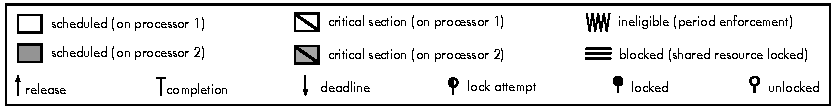
\includegraphics[scale=1]{../figures/locking/legend.pdf}
  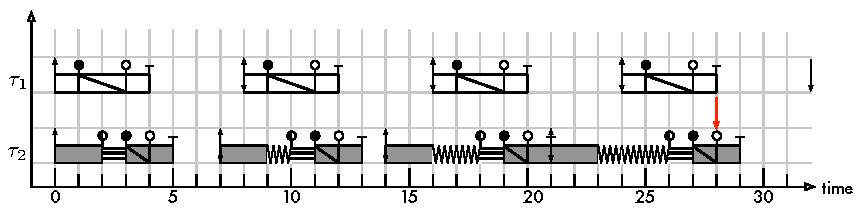
\includegraphics[scale=1]{../figures/locking/sched-locking-alt1.pdf}
  \caption{Example schedule of two tasks $\tau_1$ and $\tau_2$ on two processors sharing one lock-protected resource. The example assumes that lock requests take effect only when the critical section segment  becomes eligible to be scheduled according to the rules of the period enforcer algorithm. Under this interpretation, the fourth job of task $\tau_2$ misses its deadline at time $28$.}
  \label{fig:locking-alt1}
  \end{figure}
\fi

Since $\tau_2$'s first job requests the shared resource only after two time units of execution, it is blocked by $\tau_1$'s critical section, which commenced at time $1$. At time $3$, $\tau_1$ releases the shared resource and $\tau_2$ consequently resumes (i.e., $a^2_{2,1} = 3$). According to the period enforcer rules~\cite{Raj:suspension1991}, the second segment is immediately eligible because, according to Equation~\ref{eq:ET-def},
\begin{align*}
	ET_{2,1}^2 & = \max\left(ET_{2,0}^2 + T_2,\ \mathit{busy}(\tau_2, a^2_{2,1})\right) =\max(-T_2 + T_2,\ 3) = 3.
\end{align*}
(Recall that $ET_{2,0}^2 = -T_2$, and interpret $\mathit{busy}(\tau_2, a^2_{2,1})$ with respect to $\tau_2$'s processor.)


At time $7$, the second job of $\tau_2$ is released. Its first segment ends at time $9$. However, its second segment is not eligible to be scheduled before time $10$ since $ET_{2,2}^2 \geq ET_{2,1}^2 + T_2 = 3 + 7 = 10$. At time $9$, the second job of $\tau_1$, released at time $8$, can thus lock the shared resource without contention. Consequently, when $\tau_2$'s request for the shared resource takes effect at time $10$, the resource is no longer available and $\tau_2$ must wait until time $a^2_{2,2} = 11$ before it can proceed in its execution. We thus have
\begin{align*}
	ET_{2,2}^2 & = \max\left(ET_{2,1}^2 + T_2,\ \mathit{busy}(\tau_2, a^2_{2,2})\right) =\max(10,\ 11) = 11.
\end{align*}

The third job of $\tau_2$ is released at time $14$. Its first segment ends at time $16$, but since $ET_{2,3}^2 \geq ET_{2,2}^2 + T_2 = 11 + 7 = 18$, the second segment may not commence execution until time~$18$ and the shared resource remains available to other tasks in the meantime. The third job of $\tau_1$ is released at time $16$ and acquires the uncontested shared resource at time $17$. Thus, the segment of $\tau_2$ cannot resume execution before time $a^2_{2,3} = 19$. Therefore
\begin{align*}
	ET_{2,3}^2 & = \max\left(ET_{2,2}^2 + T_2,\ \mathit{busy}(\tau_2, a^2_{2,3})\right) =\max(18,\ 19) = 19.
\end{align*}

The same pattern repeats for the fourth job of $\tau_2$, released at time $21$: when its first segment ends at time $23$, the second segment is not eligible to commence execution before time $26$ since $ET_{2,4}^2 \geq ET_{2,3}^2 + T_2 = 19 + 7 = 26$. By then, however, $\tau_1$ has already locked the shared semaphore again, and the second segment of the fourth job of $\tau_2$ cannot resume before time $a^2_{2,4} = 27$, at which point
\begin{align*}
	ET_{2,4}^2 & = \max\left(ET_{2,3}^2 + T_2,\ \mathit{busy}(\tau_2, a^2_{2,4})\right) =\max(26,\ 27) = 27.
\end{align*}
However, this leaves insufficient time to meet the job's deadline: as the second segment of $\tau_2$ requires $C_{2,2} = 2$ time units to complete, the job's deadline at time~$28$ is  missed.

By construction, this example does not depend on a specific locking protocol; for instance, the effect occurs with both the MPCP~\cite{Ra:90} (based on priority queues) and the FMLP~\cite{BLBA:07,BA:08} (based on FIFO queues).  The corresponding response-time analyses for both protocols~\cite{Br:13,LNR:09} predict a worst-case response time of $6$ for task $\tau_2$ (i.e., four time units of execution, and at most two time units of blocking due to the critical section of $\tau_1$). 
This demonstrates that, under the first interpretation, adding period enforcement to suspension-based locks invalidates existing blocking analyses. Furthermore, it is clear that the devised repeating pattern can be used to construct schedules in which the response time of $\tau_2$  grows beyond any given implicit or constrained deadline.

Next, we show that the second interpretation can also lead to deadline misses in otherwise trivially schedulable task sets.

\subsection{Case 2: Locking Takes Effect Immediately}
 From now on, we assume the second interpretation: all lock requests are processed immediately when they are made, even if this causes the shared resource to be locked by a task that is not yet eligible to execute according to  the rules of the period enforcer algorithm. We construct an example that demonstrates \emph{unbounded} response-time growth.

To this end, consider two tasks with identical parameters hosted on two processors. Task $\tau_1$ is hosted on processor~1; task $\tau_2$ is hosted on processor~2. Both tasks have the same period and relative deadline $T_1 = T_2 = D_1 = D_2 = 8$ and the same WCET of $C_1 = C_2 = 4$. They both access a single shared resource for two time units each per job. Both tasks request the shared resource after executing for \emph{at most} one time unit. They both thus have two segments each with parameters $C_{1,1} = C_{2,1} = 1$ and $C_{1,2} = C_{2,2} = 3$. 

The example exploits that a job may require \emph{less} service than its task's specified WCET. To ensure that the shared resource is acquired in a certain order, we assume the following deterministic pattern of the actual execution times. Let $\epsilon$ be an arbitrarily small, positive real number with $\epsilon <1$. 
\begin{itemize}
	\item The first segment of even-numbered jobs  of $\tau_1$ executes for only $1-\epsilon$ time units.
	\item The first segment of odd-numbered jobs of $\tau_2$ executes for only $1-\epsilon$ time units.
%	the \nth{1}, \nth{3}, \nth{5}, \ldots, $(2i-1)$\xth job of , $\forall i=1,2,\ldots$.
%	the \nth{2}, \nth{4}, \nth{6}, \ldots, $(2i)$\xth jobs, $\forall i=1,2,\ldots$.
	\item All other segments execute for their specified worst-case costs.
\end{itemize}
Figure~\ref{fig:locking-alt2} shows an example schedule assuming periodic job arrivals.


At time $1-\epsilon$, the first job of $\tau_2$ acquires the shared resource because $\tau_1$ does not issue its request until time $1$. Consequently, $\tau_1$ is blocked until time $a^2_{1,1} = 3 - \epsilon$, and we have
\begin{align*}
	ET_{1,1}^2 & = \max\left(ET_{1,0}^2 + T_1,\ \mathit{busy}(\tau_1, a^2_{1,1})\right) =\max(-T_1 + T_1,\ 3 - \epsilon) = 3 - \epsilon
\\ \intertext{and}
	ET_{2,1}^2 & = \max\left(ET_{2,0}^2 + T_2,\ \mathit{busy}(\tau_2, a^2_{2,1})\right) =\max(-T_2 + T_2,\ 0) = 0.
\end{align*}

The roles of the second jobs of both tasks are reversed: since the second job of $\tau_1$ locks the shared resource already at time $9-\epsilon$, $\tau_2$ is blocked when it attempts to lock the resource at time~$9$. However, according to the rules of the period enforcer algorithm, the second segment of the second job of $\tau_1$ is not actually eligible to execute before time $11 - \epsilon$ since
\begin{align*}
	ET_{1,2}^2 & = \max\left(ET_{1,1}^2 + T_1,\ \mathit{busy}(\tau_1, a^2_{1,2})\right) =\max(3 - \epsilon + 8,\ 8) = 11 - \epsilon.
\end{align*}
Consequently, even though the lock is granted to $\tau_1$ already  at time $9-\epsilon$, the critical section is executed only starting at time $11 - \epsilon$, and $\tau_2$ is thus delayed until time $13 - \epsilon$. At time $13 - \epsilon$, $\tau_2$ is immediately eligible to execute since
\begin{align*}
	ET_{2,2}^2 & = \max\left(ET_{2,1}^2 + T_2,\ \mathit{busy}(\tau_2, a^2_{2,2})\right) =\max(0 + 8,\ 13 - \epsilon) = 13 - \epsilon.
\end{align*}

The third jobs of both tasks are released at time $16$. The roles are swapped again: because $\tau_2$'s first segment requires only $1-\epsilon$ time units of service, it acquires the lock at time $a^2_{2,3} = 17 - \epsilon$, before $\tau_1$ issues its request at time~$17$. However, according to the period enforcer algorithm's eligibility criterium, $\tau_2$ cannot actually continue its execution before time $21- \epsilon$ since
\begin{align*}
	ET_{2,3}^2 & = \max\left(ET_{2,2}^2 + T_2,\ \mathit{busy}(\tau_2, a^2_{2,3})\right) =\max(13- \epsilon + 8,\ 16) = 21- \epsilon.
\end{align*}
This, however, means that $\tau_1$ cannot use the shared resource before time $23 - \epsilon$, which leaves insufficient time to complete the second segment of $\tau_1$'s third job before its deadline at time $24$.
Furthermore, if both tasks continue the illustrated execution pattern, the period enforcer continues to increase their response times. As a result,  unbounded worst-case response times may arise. 

As in the previous example,  the response-time analyses for both the MPCP~\cite{Br:13,LNR:09} and the   FMLP~\cite{Br:13} predict a worst-case response time of $6$ for both tasks (i.e., four time units of execution, and at most two time units of blocking). The example thus demonstrates that, if lock requests take effect immediately, then the period enforcer is incompatible with existing blocking analyses because, under the second interpretation, it increases the effective lock-holding times.


\ifpaper
\begin{figure}[t]
  \centering
  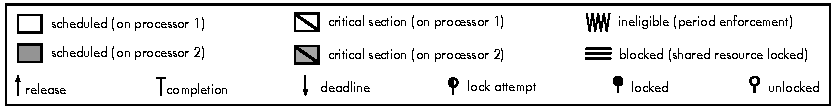
\includegraphics[scale=1]{../figures/locking/legend.pdf}
  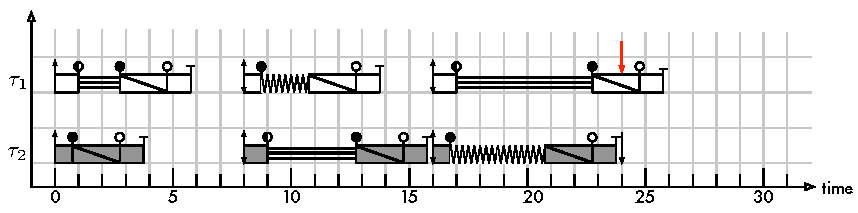
\includegraphics[scale=1]{../figures/locking/sched-locking-alt2.pdf}
  \caption{Example schedule of two tasks $\tau_1$ and $\tau_2$ on two processors sharing one lock-protected resource. The example assumes that lock requests take effect immediately, even if the critical section segment is not yet eligible to be scheduled according to the rules of the period enforcer algorithm. Under this interpretation, the third job of task $\tau_1$ misses its deadline at time $24$.}
  \label{fig:locking-alt2}
  \end{figure}
\fi

\subsection{Discussion}

While it is intuitively appealing to combine period enforcement with suspension-based locking protocols, we observe that this causes non-trivial difficulties. In particular, our examples show that the addition of period enforcement invalidates all existing blocking analyses. They also suggest that devising a correct blocking analysis would be a substantial challenge due to the demonstrated feedback cycle between the period enforcer rules and blocking durations. 


Fundamentally, the design of the period enforcer algorithm implicitly rests on the assumption that a segment \emph{can} execute as soon as it is eligible to do so. In the presence of locks, however, this assumption is invalidated. As demonstrated, the result can be a successive growth of self-suspension times that proceeds until a deadline is missed.  The period enforcer algorithm, at least as defined and used in the literature to date~\cite{Raj:suspension1991,Raj:91}, is therefore incompatible with the existing literature on suspension-based real-time locking protocols (e.g., \cite{Raj:91,Lak:11,LNR:09,BLBA:07,Br:13}). 


Finally, it is worth noting that our examples can be trivially extended with lower-priority tasks to ensure that no processor idles before the described deadline misses occur. It is also not difficult to extend the second example with a task on a third processor such that all segments of $\tau_1$ and $\tau_2$ are separated by a non-zero self-suspension.


\section{Concluding Remarks}
\label{sec:conclusion}

We have revisited the underlying assumptions and limitations of the period enforcer algorithm, which Rajkumar \cite{Raj:suspension1991} introduced to handle segmented self-suspending real-time tasks. 

One key assumption in the original proposal \cite{Raj:suspension1991} is that a deferrable task $\tau_i$ can defer its entire execution time but not parts of it. This creates some mismatches between the original self-suspending task set and the corresponding deferrable task set, which we have demonstrated with an example that shows that Theorem 5 in \cite{Raj:suspension1991} does not reflect the schedulability of the original self-suspending task system. 


Furthermore, the original proposal \cite{Raj:suspension1991} left open the question of how to convert a segmented self-suspending task set to a corresponding set of deferrable tasks. Taking into account recent developments~\cite{ecrts15nelissen}, we have observed that such a task set transformation is non-trivial in the general case.  

Finally, we have demonstrated that substantial difficulties arise if one attempts to combine suspension-based locks with period enforcement. These difficulties stem from the fact that period enforcement can increase contention or lock-holding times, which increases the lengths of self-suspension intervals, which then in turn feeds back into the period enforcer's minimum suspension lengths. As a consequence, period enforcement invalidates all existing blocking analyses.

Nevertheless, Theorem 5 in \cite{Raj:suspension1991} could be useful for handling self-suspending tasks (that do not use suspension-based locks) if there exist \emph{efficient} schedulability tests for the corresponding deferrable task systems or the period enforcer algorithm. However, such tests have not been found yet and the development of a precise and efficient schedulability test for self-suspending tasks remains an open problem.


\section*{Acknowledgements}

We thank James H.\ Anderson and Raj Rajkumar for their comments on drafts of this paper.
This paper has been supported by DFG, as part of the Collaborative
Research Center SFB876 (http://sfb876.tu-dortmund.de/).

\bibliography{../bibliography/biblio}{}

\end{document}
